\documentclass[12pt, a4paper, openany]{book}
\usepackage[inline]{enumitem}
\usepackage{../generalStyle}
\usepackage{amsmath}

\graphicspath{ {./img/} }

\begin{document}

\title{Ricerca Operativa e Pianificazione delle Risorse}
\author{
	Fabio Ferrario\\
	\small{\href{https://t.me/fefabo}{@fefabo}}
	\\\\Sara Angeretti\\
	\small{\href{https://t.me/Sara1798}{@Sara1798}}
}
\date{2022/2023}
\maketitle

\tableofcontents

\input{chapters/introduzione}

\input{chapters/prerequisiti}

\input{chapters/modelli_nella_ricerca_operativa}

\input{chapters/metodo_del_simplesso}

\input{chapters/dualità}

\input{chapters/modelli_pli}

\input{chapters/branchandbound}

\input{chapters/programmazione_non_lineare}

\documentclass[12pt, a4paper, openany]{book}
\usepackage[inline]{enumitem}
\usepackage{../generalStyle}
\usepackage{amsmath}

\graphicspath{ {./img/} }

\begin{document}

\chapter{Assignments}

\section{Assignment 1}

\subsection{Soluzione grafica}
\begin{center}
    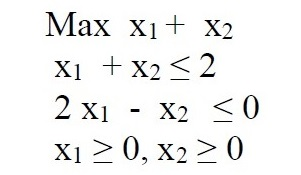
\includegraphics[width=0.325\textwidth]{Assignment1_es1Q.jpg}
\end{center}
\begin{center}
    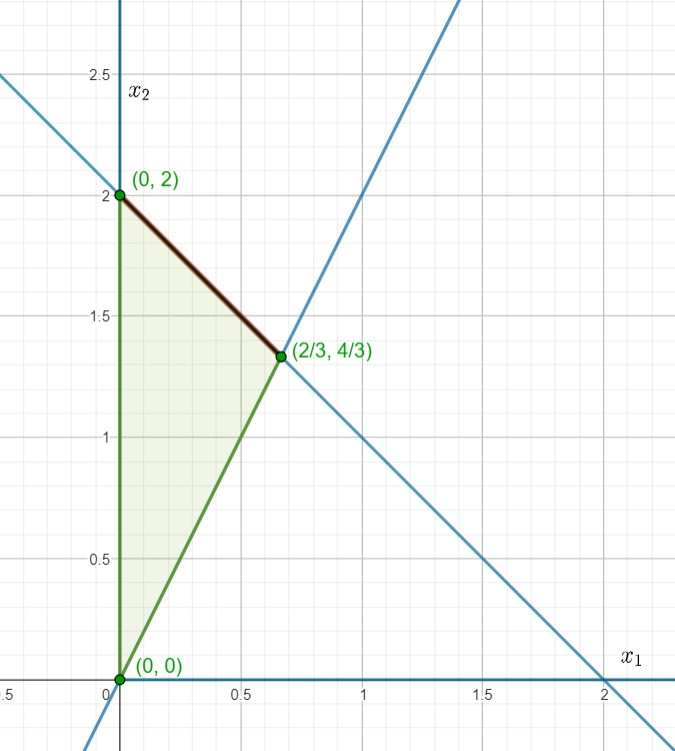
\includegraphics[width=0.5\textwidth]{Assignment1_es1A.jpg}
\end{center}
\vspace{1cm}

\subsection{Soluzione con Metodo del Simplesso}
\begin{center}
    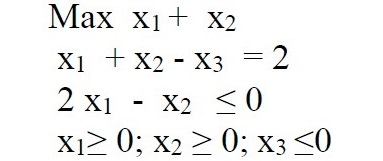
\includegraphics[width=0.325\textwidth]{Assignment1_es2Q.jpg}
\end{center}
\begin{flalign*}
    Z\ =\ &\ x_1 + x_2 \\
        &\ x_1 + x_2 - x_3 = 2 \\
        &\! 2x_1 - x_2\qquad\ \leq 0 \\
        \\
        &\ x_1 \geq 0,\ x_2 \geq 0,\ x_3 \leq 0 &&
\end{flalign*}
\begin{flalign*}
    Z\ -\ &\ x_1 - x_2 = 0 \\
        &\ x_1 + x_2\ \textcolor{blue}{\mathbf{+\ x'_3}}\ = 2 \\
        &\! 2x_1 - x_2\ \qquad\ \ \leq 0 \\
        \\
        &\ x_1 \geq 0,\ x_2 \geq 0,\ \textcolor{blue}{\mathbf{x'_3 \geq}\ 0} &&
\end{flalign*}
\begin{flalign*}
    Z\ -\ &\ x_1 - x_2 = 0 \\
        &\ x_1 + x_2 + x'_3\ \qquad \ = 2 \\
        &\! 2x_1 - x_2\qquad\ \textcolor{blue}{\mathbf{+\ x_4}\ =}\ 0 \\
        \\
        &\ x_1 \geq 0,\ x_2 \geq 0,\ x'_3 \geq 0,\ \textcolor{blue}{x_4 \geq 0} &&
\end{flalign*}

\noindent Se l'origine del problema $(0,\ 0)$ è ammissibile, seleziono $x_1$ e $x_2$ (cioè le variabili della funzione obiettivo) come \textbf{variabili di base}.\\
\noindent Provo il problema originario usando l'\textbf{origine del problema}, ovvero azzero $x_1$ e $x_2$.\\
\\
\noindent Iterazione 0:
\begin{center}
    \begin{tabularx}{0.75\textwidth}{ |c|X|X|X|X|X|X|c| } 
        \hline
        Var di Base & Eq & $Z$ & $x_1$ & $x_2$ & $x'_3$ & $x_4$ & t. n.\\
        \hline 
        \hline 
        $Z$ & R$_0$ & 1 & -1 & -1 & 0 & 0 & 0\\
        \hline 
        $x'_3$ & R$_1$ & 0 & 1 & 1 & 1 & 0 & 2\\
        \hline 
        $x_4$ & R$_2$ & 0 & 2 & -1 & 0 & 1 & 0\\
        \hline
    \end{tabularx}
\end{center}

\noindent I vincoli sono rispettati. Ottengo dunque la \textbf{soluzione di base ammissibile} $(0,\, 0,\ 2,\ 0)$.\\
La soluzione di base che ho ottenuto è \textbf{ottimale}? Lo è se nella riga R$_0$ corrispondente alla funzione obiettivo ho solo coefficienti \textbf{\textit{non} negativi}.\\
\noindent Ho $-1$ e $-1$, quindi \textbf{non} è ottimale. Allora procedo.\\

\noindent Ora scelgo la \textit{variabile non di base \textbf{entrante}}. Di solito è quella con coefficiente con \textit{valore assoluto \textbf{maggiore}}. Ma qui ho $-1$ e $-1$ quindi scelgo in maniera arbitraria.\\
\noindent \underline{Scelgo $x_1$}, la cui colonna diventa \textbf{colonna pivot}. La \textbf{riga pivot} viene identificata tramite la \textbf{\textit{regola del rapporto minimo}}. Questa mi dà un numero che corrisponde al rapporto fra il \textbf{termine noto} e il coefficiente della \textbf{variabile entrante} che ho già individuato.\\
\noindent Nel nostro caso $x'_3$ mi dà $\frac{2}{1}$ e $x_4$ mi dà ($\frac{0}{2}$), perciò $x_4$ vince la regola del rapporto minimo diventando la \textit{variabile \textbf{uscente}}. Ricapitolando, $x_1$ è la \textit{variabile \textbf{entrante}} e $x_4$ è la \textit{variabile \textbf{uscente}}, mentre il \textit{\textbf{numero pivot}} è 2.\\
\noindent Ricorda la regola:
\begin{center}
    \noindent Prima divido la riga pivot $R_p$ per il numero pivot.\\ Poi tutte le altre righe con la formula:
\end{center}
\begin{center}
    $R_i = R_i - |c|\cdot R_p$\qquad se\ $c > 0$\\
\end{center}
\begin{center}
    $R_i = R_i + |c|\cdot R_p$\qquad se\ $c < 0$\\
\end{center}

\noindent Procedo con la prossima iterazione.\\
\\
\noindent Iterazione 1:
\begin{center}
    \begin{tabularx}{0.75\textwidth}{ |c|X|X|X|X|X|X|c| } 
        \hline
        Var di Base & Eq & $Z$ & $x_1$ & $x_2$ & $x'_3$ & $x_4$ & t. n.\\
        \hline
        \hline
        $Z$ & R$_0$ & 1 & 0 & $-\frac{3}{2}$ & 0 & $\frac{1}{2}$ & 0\\
        \hline 
        $x'_3$ & R$_1$ & 0 & 0 & $\frac{3}{2}$ & 1 & $-\frac{1}{2}$ & 2\\
        \hline 
        $x_1$ & R$_2$ & 0 & 1 & $-\frac{1}{2}$ & 0 & $\frac{1}{2}$ & 0\\
        \hline
    \end{tabularx}
\end{center}
\noindent La soluzione di base ammissibile che ottengo è $(0,\ 0,\ 2,\ 0)$, la stessa di prima. Procedo dunque con il prossimo passo.\\
\noindent Questa volta la \textit{variabile \textbf{entrante}} è $x_2$ perché è l'unica con coefficiente \textbf{negativo} nella riga della funzione obiettivo.\\
\noindent Invece la \textit{variabile \textbf{uscente}} è $x'_3$ perché è l'unica con coefficiente \textbf{positivo} nella colonna della \textit{variabile entrante}. Il nuovo \textbf{numero pivot} è $\frac{3}{2}$.\\
\\
\noindent Iterazione 2:
\begin{center}
    \begin{tabularx}{0.75\textwidth}{ |c|X|X|X|X|X|X|c| } 
        \hline
        Var di Base & Eq & $Z$ & $x_1$ & $x_2$ & $x'_3$ & $x_4$ & t. n.\\
        \hline
        \hline
        $Z$ & R$_0$ & 1 & 0 & 0 & 1 & 0 & 2\\
        \hline 
        $x'_3$ & R$_1$ & 0 & 0 & 1 & $\frac{2}{3}$ & $-\frac{1}{3}$ & $\frac{4}{3}$\\
        \hline 
        $x_1$ & R$_2$ & 0 & 1 & 0 & $\frac{1}{3}$ & $\frac{1}{3}$ & $\frac{2}{3}$\\
        \hline
    \end{tabularx}
\end{center}

\noindent La soluzione di base ammissibile che ottengo è $(\frac{2}{3},\ \frac{4}{3},\ 0,\ 0)$ e $Z$ ha valore $Z\ =\ 2$. Procedo controllando se è una soluzione ottimale.\\
\noindent Ho tutti coefficienti non negativi nella riga della funzione obiettivo, quindi \textbf{la mia soluzione è ottimale}. Esercizio finito.\\
\noindent Però nota bene: all'inizio ho fatto una scelta arbitraria, scegliendo $x_1$ come variabile non di base entrante. Cosa succederebbe se scegliessi invece $x_2$?\\
\\
\noindent \textbf{Ricomincio l'esercizio scegliendo $x_2$ come variabile non di base entrante}.\\
\\
\noindent Iterazione 0:
\begin{center}
    \begin{tabularx}{0.75\textwidth}{ |c|X|X|X|X|X|X|c| } 
        \hline
        Var di Base & Eq & $Z$ & $x_1$ & $x_2$ & $x'_3$ & $x_4$ & t. n.\\
        \hline 
        \hline 
        $Z$ & R$_0$ & 1 & -1 & -1 & 0 & 0 & 0\\
        \hline 
        $x'_3$ & R$_1$ & 0 & 1 & 1 & 1 & 0 & 2\\
        \hline 
        $x_4$ & R$_2$ & 0 & 2 & -1 & 0 & 1 & 0\\
        \hline
    \end{tabularx}
\end{center}
\noindent \textit{Variabile entrante}: $x_2$.\\
\noindent \textit{Variabile uscente}: $x'_3$, ovvero l'unica con coefficiente positivo nella colonna della variabile entrante.\\
\noindent \textit{Numero pivot}: $1$.\\
\\
\noindent Iterazione 0:
\begin{center}
    \begin{tabularx}{0.75\textwidth}{ |c|X|X|X|X|X|X|c| } 
        \hline
        Var di Base & Eq & $Z$ & $x_1$ & $x_2$ & $x'_3$ & $x_4$ & t. n.\\
        \hline 
        \hline 
        $Z$ & R$_0$ & 1 & 0 & 0 & 1 & 0 & 2\\
        \hline 
        $x'_3$ & R$_1$ & 0 & 1 & 1 & 1 & 0 & 2\\
        \hline 
        $x_4$ & R$_2$ & 0 & 3 & 0 & 1 & 1 & 2\\
        \hline
    \end{tabularx}
\end{center}

\noindent La soluzione di base ammissibile che ottengo è $(0,\ 2,\ 0,\ 2)$ e $Z$ ha valore $Z\ =\ 2$. Procedo controllando se è una soluzione ottimale.\\
\noindent Ho solo coefficienti non negativi nella riga della funzione obiettivo, perciò \textbf{la mia soluzione è ottimale}.\\
\noindent Però con $x_1$ avevo ottenuto una soluzione ottimale diversa, ovvero $(\frac{2}{3},\ \frac{4}{3},\ 0,\ 0)$. Va bene? Sì se questi due vertici sono \textit{adiacenti}.\\
\noindent Ma \textbf{quando due vertici sono adiacenti? Quando condividono $n\ -\ 1$ \textit{frontiere di vincoli}}.\\
\noindent Contando di non aver fatto errori nei tableau, posso assumere che lo siano. In tal caso \textit{la mia soluzione ottimale sarà il \textbf{segmento} che unisce i due vertici} $(0,\ 2,\ 0,\ 2)$ \textit{e} $(\frac{2}{3},\ \frac{4}{3},\ 0,\ 0)$ \textit{e che avrà come valore della funzione obiettivo} $Z\ =\ 2$.\\
\\
\noindent \textbf{\textit{Però potrei avere una domanda per Fabio: ho letto nel tuo file che due vertici sono adiacenti se condividono tutte le variabili non di base tranne una. Io qua ho}} $(0,\ 2,\ 0,\ 2)$ \textbf{\textit{che ha come variabili non in base}} $x'_3$ \textbf{\textit{e}} $x_4$ \textbf{\textit{mentre}} $(\frac{2}{3},\ \frac{4}{3},\ 0,\ 0)$ \textbf{\textit{ha come variabili in base}} $x_2$ \textbf{\textit{e}} $x_4$. \textbf{\textit{La mia domanda è: condividono}} $x_2$, \textbf{\textit{basta per dire che sono adiacenti o devono condividere il valore}}?



\end{document}

\end{document}
